\section{Explaining deep graph models}
\label{s_ExplainingGNNs}

%No longer purely related work. First outline explainable ai in general, then transition to gnns and the cummulate into the next chapter on explanability methods on gnns. Last part of the chapeter is the related work subchapter

% Introduction into related work, laying out the general story of the chapter: From explanations on static graphs and the different approaches to more detailed description of highly related work on explanations on dynamic graphs

Alongside the rise in adaptation of artificial intelligence, and deep learning methods over recent years, the idea of explainable artificial intelligence has been gaining increasing attention \cite{adadi_peeking_2018}. This field of research focuses on providing transparency over the mechanisms that underlie such artificial models \cite{barredo_arrieta_explainable_2020}. Many machine learning models behave like a \textit{black-box}, meaning that the mechanisms that lead to their predictions remain opaque to their users \cite{prado-romero_survey_2023}. Explainable artificial intelligence differentiates \textit{interpretability}, the degree to which the inner structures of a model are understandable to a human by design \cite{barredo_arrieta_explainable_2020, li_explainability_2022}, from \textit{explainability}, actions taken by a model aiming to explain its internal mechanisms \cite{barredo_arrieta_explainable_2020}. While interpretable models utilize mechanisms that are easy to understand on their own \cite{prado-romero_survey_2023}, black-box models have shown better performance on high-dimensional input data \cite{prado-romero_survey_2023}. Thus, a multitude of approaches that aim to explain such black-box models have been investigated \cite{barredo_arrieta_explainable_2020, adadi_peeking_2018}.

%Transition to explanability for gnns and outline the structure of this chapter.

Even though most works on \glspl{gnn} have only emerged in the past 10 years \cite{wu_comprehensive_2021}, the black-box nature of most of these \glspl{gnn} gave rise to a plethora of explanation methods. The proposed approaches vary in many ways, like the type of explanation provided, how the explained model is used, or if and how explainers are trained \cite{kakkad_survey_2023}. Figure \ref{f_taxonomy_explainers} provides a classification of these varied approaches. At the conceptual level, we follow the categorization proposed by Yuan et al. \cite{yuan_explainability_2020}, which distinguishes between model-level and instance-level approaches. Model-level methods explain \glspl{gnn} as a whole, irrespective of any particular input example \cite{yuan_explainability_2020}. Such explanations aim to uncover a high-level understanding of the inner workings of the explained \gls{gnn}. In comparison, instance-level methods explain the model output for a specific input \cite{yuan_explainability_2020}. These explanations are tailored to individual instances, offering a fine-grained understanding of the reasoning behind each prediction.

\begin{figure}[ht]
    \centering
    \tikzset{
  basic/.style  = {draw, rectangle, minimum height=7.5mm, outer sep=0},
  root/.style   = {basic, thin, align=center},
  level 2/.style = {basic, thin, align=center, sibling distance=60mm, text width=10em},
  level 3/.style = {basic, thin, align=center, sibling distance=30mm, text width=10em},
  level 4/.style = {basic, thin, align=center, text width=7.5em}
}
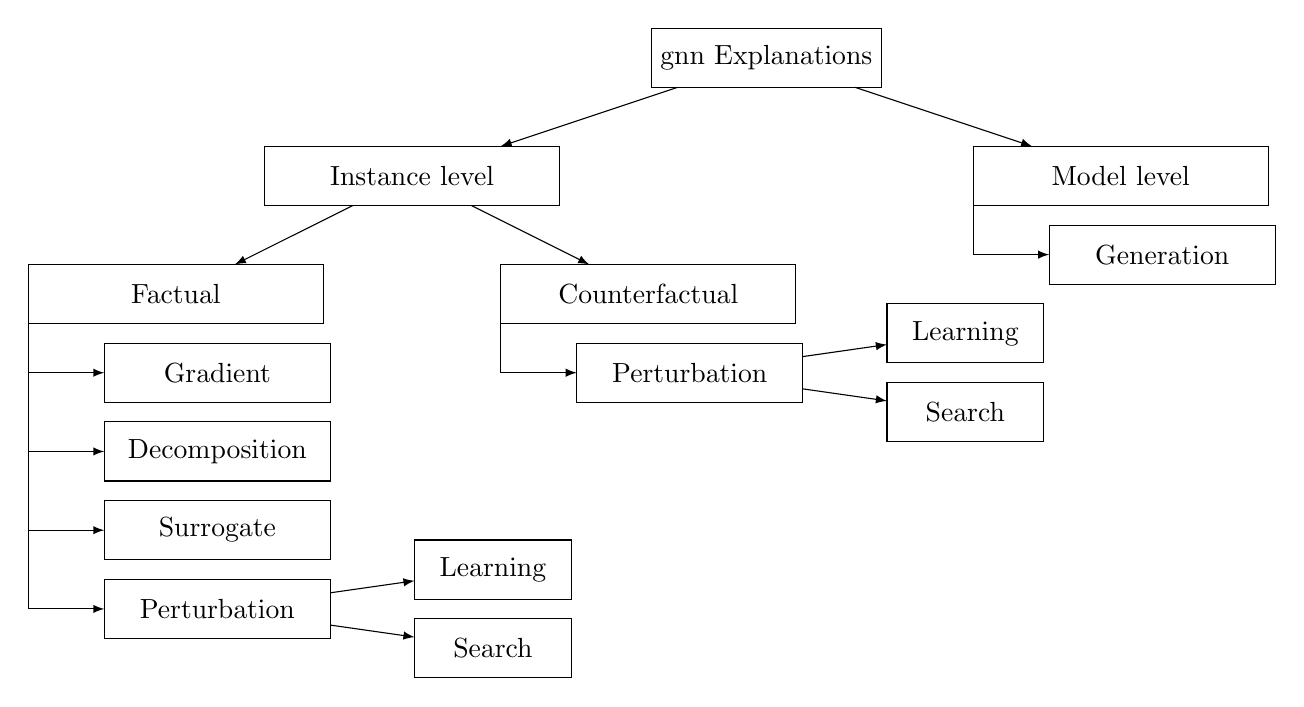
\begin{tikzpicture}[level 1/.style={sibling distance=90mm}, edge from parent/.style={->,draw}, >=latex]
    \node[root] {\gls{gnn} Explanations}
        child {node[level 2] (c1) {Instance level}
            child {node[level 3] (c3) {Factual}}
            child {node[level 3] (c4) {Counterfactual}}
        }
        child {node[level 2] (c2) {Model level}};

    \begin{scope}[every node/.style={level 4}]
        \node[below of = c3, xshift=15pt] (c31) {Gradient};
        \node[below of = c31] (c32) {Decomposition};
        \node[below of = c32] (c33) {Surrogate};
        \node[below of = c33] (c34) {Perturbation};

        \node[right of = c34, text width=5em, xshift=2.5cm, yshift = 0.5cm] (c341) {Learning};
        \node[below of = c341, text width=5em] (c342) {Search};

        \node[below of = c4, xshift=15pt] (c41) {Perturbation};

        \node[right of = c41, text width=5em, xshift=2.5cm, yshift = 0.5cm](c411){Learning};
        \node[below of = c411, text width=5em](c412){Search};

        \node[below of = c2, xshift=15pt] (c21) {Generation};
    \end{scope}

    \draw[->] (c34) -- (c341);
    \draw[->] (c34) -- (c342);

    \draw[->] (c41) -- (c411);
    \draw[->] (c41) -- (c412);

    \foreach \value in {1,...,4}
        \draw[->] (c3.188) |- (c3\value.west);
    \foreach \value in {1}
        \draw[->] (c4.188) |- (c4\value.west);
    \foreach \value in {1}
        \draw[->] (c2.188) |- (c2\value.west);
\end{tikzpicture}
    \caption{Taxonomy of \gls{gnn} explanation methods. Explanation approaches are categorized into instance-level and model-level methods. The category of instance-level methods is further subdivided into factual and counterfactual approaches. Taxonomy adapted from \cite{yuan_explainability_2020}, \cite{prado-romero_survey_2023}, and \cite{kakkad_survey_2023}.}
    \label{f_taxonomy_explainers}
\end{figure}

\textit{Model-level} explainers like XGNN \cite{yuan_xgnn_2020} map the behavior of a \gls{gnn} to patterns in the input graphs \cite{yuan_explainability_2020}. In the generation approach, \glspl{gnn} are explained by training a model to generate graphs that maximize a particular prediction of the \gls{gnn} \cite{yuan_explainability_2020, yuan_xgnn_2020}. The thereby generated graph patterns are then used as an explanation \cite{yuan_xgnn_2020}. While these approaches can provide high-level explanations for the general model behavior, they fail to explain the specifics of why a certain prediction has been made for a given input and are thus not discussed any further.

\textit{Instance-level} approaches are subdivided into those that provide a factual and those that provide a counterfactual explanation. On a fundamental level, factual reasoning inquires, "With A already having occurred, will B occur?" \cite{quelhas_relation_2018, tan_learning_2022}. In contrast, counterfactual reasoning poses the question, "If A did not occur, would B still happen?" \cite{quelhas_relation_2018, tan_learning_2022}. The following sections take a closer look at explanation methods using either type of reasoning.

\subsection{Factual Explanation Approaches}
\label{s_ExplainingGNNs_Factual}

Factual explanations for \glspl{gnn} answer the question: "Given the input A, will the \gls{gnn} predict B?". These explanations seek the input information with the maximum influence on the \gls{gnn}'s prediction \cite{kakkad_survey_2023}. They can take the form of a subgraph $G' \subseteq G$ of the original input $G$ \cite{kakkad_survey_2023} that is considered \textit{sufficient} to produce the original prediction by the \gls{gnn} $f(\cdot)$ \cite{tan_learning_2022} if the following equation holds:

\begin{equation}
    f(G) = f(G')
\end{equation}

Factual explainers for \glspl{gnn} are categorized based on the primary mechanisms they employ to explain predictions, each offering different approaches and forms of explanations:

\begin{itemize}
    \item \textbf{Gradient/Feature} based methods identify important features by analyzing how changes in input features affect the network's predictions \cite{yuan_explainability_2020}. These approaches either employ back-propagation to examine the gradients of the explained prediction concerning the input features or map hidden features through interpolation into the input space \cite{yuan_explainability_2020}.
    \item \textbf{Decomposition} methods break down the \gls{gnn}'s prediction into contributions from individual nodes or edges by creating score decomposition rules through back-propagation \cite{yuan_xgnn_2020}. These rules attribute the prediction scores to individual features in the input space \cite{yuan_explainability_2020}.
    \item \textbf{Surrogate} methods create a separate, easy-to-interpret model to approximate the behavior of the \gls{gnn} on data similar to the explained example \cite{yuan_explainability_2020}. Usually, neighboring data to the explained example is sampled and used to train easily analyzable models \cite{yuan_explainability_2020} like linear regression models \cite{duval_graphsvx_2021} or Bayesian networks \cite{vu_pgm-explainer_2020}.
    \item \textbf{Perturbation} based methods analyze how the model output changes when the input is perturbed \cite{yuan_explainability_2020}. These methods usually create feature masks that highlight the input features important for the prediction \cite{yuan_explainability_2020, ivanovs_perturbation-based_2021}.
\end{itemize}

While gradient/feature and decomposition approaches require direct access to the internal model parameters or embeddings by design, some surrogate and perturbation based methods can operate without such access \cite{kakkad_survey_2023}. Needing direct access is a disadvantage since it requires adaptations in the explainer before it can be applied to new models and prohibits the application of the explainers to models that do not expose their inner workings.

Perturbation-based methods operate with either a learning-based or a search-based perturbation approach \cite{xia_explaining_2023}. Learning-based approaches identify the most critical features of the input graph by feeding the node embeddings and/or edge embeddings produced by the explained \gls{gnn} into a learnable model that extracts a perturbed subgraph \cite{kakkad_survey_2023, xia_explaining_2023}. The \gls{gnn} predictions on this subgraph are then compared to the original predictions with a distance function, providing a score that serves as training input for the subgraph extraction model \cite{kakkad_survey_2023}. Search-based perturbation approaches generate modified subgraphs from the original input using heuristic search algorithms together with a game-theoretical scoring function \cite{xia_explaining_2023, yuan_explainability_2021}. A clear advantage of the search-based perturbation strategy is that model access is only needed on the level of predictions, not for the embeddings. This comes at the cost of longer inference times \cite{xia_explaining_2023} since the search-based approach requires the explicit exploration of various input perturbations.

% Write something to put these methods into perspective. For example a disctinction between search- and learning-based perturbation approaches should be included since I refer to it in the related work section

% Idea would be to compare these 4 approaches and to discuss their most interesting characteristics and shortcomings. I wonder if it makes sense to actually detail the inner workings of any particular explainer or not because it is only inderectly relevant to my thesis

\subsection{Counterfactual Explanation Approaches}
\label{s_ExplainingGNNs_CounterFactual}

Counterfactual explanations for \glspl{gnn} answer the question, "What changes in the input A are necessary for the \gls{gnn} to predict differently, no longer predicting B?". These explanations consist of the smallest possible alteration to the input information such that the model prediction changes \cite{kakkad_survey_2023}. These counterfactual explanations are often referred to as counterfactual examples and consist of the input information that is \textit{necessary} to produce the same prediction as for the complete information \cite{tan_learning_2022}. Counterfactual explanations for \glspl{gnn} have risen in attention over the last years \cite{ma_clear_2022} for their ability to produce intuitive explanations \cite{ma_clear_2022}, offer feedback for non-experts \cite{prado-romero_survey_2023}, foster trust in \glspl{gnn} \cite{prado-romero_survey_2023}, and help address model biases \cite{prado-romero_survey_2023}.

Typically, counterfactual explanations involve a subgraph $\mathcal{X} \subseteq G$, for which the explained \gls{gnn} $f(\cdot)$ produces a different prediction compared to the original graph $G$ as input when $\mathcal{X}$ is removed from $G$ \cite{tan_learning_2022}:
\begin{equation}
    \label{e_cf_explanation}
    f(G) \neq f(G\setminus \mathcal{X})
\end{equation}

In some cases, counterfactual examples also include information added to the original graph $G$. In such instances, the definition of counterfactual explanations evolves. Here, counterfactual explanations $\mathcal{X} = \{\mathcal{X}^-, \mathcal{X}^+\}$ consist of a graph $\mathcal{X}^- \subseteq G$, containing information removed from $G$, and a graph $\mathcal{X}^+ = (V^+, E^+)$ with ${v_i \in V^+ \implies v_i \notin V}$ and $e_i \in E^+ \implies e_i \notin E$ that contains information added to the input graph. This combination must satisfy the following equation:

\begin{equation}
    f(G) \neq f((G \cup \mathcal{X}^+) \setminus \mathcal{X^-})
\end{equation}

Counterfactual explainers fall into three high-level methods that differ in how they seek alterations in the input graph to create counterfactual explanations.

\begin{itemize}
    \item \textbf{Search based} approaches explore alterations to the input graph dependent on a specific criterion \cite{prado-romero_survey_2023}, like a similarity measure between graph alterations \cite{faber_contrastive_2020}, to find a counterfactual example.
    \item \textbf{Heuristic based} methods depend on a systematic policy for modifying the input graph until they attain a valid counterfactual \cite{prado-romero_survey_2023}. For instance, they may alter the original input by randomly dropping and adding edges until the prediction of the \gls{gnn} changes \cite{abrate_counterfactual_2021}.
    \item \textbf{Learning based} approaches examine how the \gls{gnn} output changes with input variations \cite{prado-romero_survey_2023}. First, a mask to highlight relevant features in the input graph is generated, which is then used to modify the input graph such that important features stay the same \cite{prado-romero_survey_2023}. This modified input graph is then fed into the \gls{gnn} again to get a score for this modification \cite{prado-romero_survey_2023}. The score is then used to update the mask for the next iteration \cite{prado-romero_survey_2023}. Various approaches within this category differ in how they create and update the input graph mask. 
\end{itemize}

These methods are not mutually exclusive, for instance there are explainers \cite{bajaj_robust_2021} that integrate learning and heuristic based approaches.

% Make the case for cf explanations over f explanations

In summary, while factual explanations shed light on why a GNN makes a particular prediction given the input, counterfactual explanations go a step further by revealing precisely what changes in the input are needed to alter that prediction. Counterfactual explanations provide a practical and intuitive way for users to grasp what influences the model's output. By offering concrete, actionable insights into the model's decision-making process, they empower individuals to understand, trust, and even improve \glspl{gnn} in real-world applications \cite{prado-romero_survey_2023}. Thus, counterfactual explanations bridge the gap between the model's black-box behavior and human interpretability, making them a valuable tool for ensuring transparency and accountability.
